
\todo {Things that need to be done for the plots}
\begin{itemize}
	\item (Plots) Shape comparisons of main analysis variables for CR3, CR2, SR (Gives the idea of the uncertainty)
	\item (Table) Cross section limits of 7 TeV studies (Just put al the numbers in the formula)
\end{itemize}


\begin{itemize}
	\item Brief introduction of the chapter content
	\item State that everything is based on the 7 TeV studies and will go in details on the differences
\end{itemize}


\section{Signal and background samples}

\begin{itemize}
	\item List of samples used for the studies
	\item brief details on how the signal samples has been generated and how data is stored now (miniaods), everything on the production chain (if too much refers to appendix)
\end{itemize}



\section{Object reconstruction and event selection}
\begin{itemize}
	\item make clear the experiment will gain access to a trigger triggering only on di-jet properties (no MET Lvl 1 seed like for 7 TeV)
	\item MET cut removed (chosen variable for cuts optimization)
	\item Dijet delta eta cut removed (obsolete because strongly correlated to the $m_{jj}$ cut) 
	\item $m_{jj}$ cut removed (chosen variable for cuts optimization), be aware of the fact that there's gonna be an online cut coming from the chosen trigger anyway.
	\item \hadtau isolation requirement has still high impact on statistics
	\item mention new b-jet and lepton veto used (reference to internal notes if necessary)
\end{itemize}

During the technical stop the experiment underwent through several updates on both hardware and software side. This	translates in an updated version of the physical object definition, therefore an improved event selection for the study with respect to the 7\tev analysis.

The \hadtau object reconstruction went through a major update with the introduction of new isolation and decay mode discriminators and electron veto \cite{bib:TauID_13tev}. The new \hadtau object reconstruction has been commissioned for $\pt > 20$\gev ad in all $\eta$ ranges. By using the specifications suggested by the Tay POG there's an increase of the overall TauID efficiency of about 10\% for loose isolated \hadtau with respect to the 7\tev specifications, going up to 71\% for $Z \longrightarrow\tau\tau$ events\cite{bib:TauID_13tev}. A detailed list of the \hadtau object selection can be found on Table \ref{table:tauobjdefinition_13TeV}.

The Jet object definition remained unchanged for those 13\tev studies.


With Run 2 the experiment will gain access to a new trigger list. The aim is to use a trigger that is exclusively making an online selection on the di-jet object kinematic properties. Differently with the 7\tev trigger version this trigger can't be seeded by a level one trigger based on \met. The drop of all online selections over the \hadtau properties leads to some important advantages Firstly it is possible to have a lower \hadtau \pt selection. Secondly it is possible to go from a 1-prong to a 3-prong decay selection since this stringent requirement is not part anymore of any level 1 trigger seed. 

\section{Sensitivity and cross section limit studies}

\begin{itemize}
	\item Optimization of cuts to exclude signal at the lowest cross section;
	\item the reference study formula is $\dfrac{S}{\sqrt{B + (0.5 \cdot B)^{2}}} > 2$
	\item signal events can also be express as: $S = \epsilon ( Pt_{\tau} , m_{jj} ,  \met )\cdot \sigma \cdot L$
	\item The sensitivity study is done as function of 3 different variables: $\tau_{pt}$, MET and $m_{jj}$
	\item Background prediction in SR: two-fold ABCD method involving 2 different (Schematic rappresentation needed) correction factors
	\item LtoT conversion factor:
	\begin{itemize}
		\item Events with at least 4 jets;
		\item $NLto2T = A * B$;
		\item A: (the matched tau is also tight isolated)/(at least one jet matched to a loose tau)
		\item B: (the matched tau is also tight isolated)/(at least one jet matched to a tau (no iso requirement))
	\end{itemize}
		\item VBF conversion factor: same as before (Excluding removed cuts)
		\item Min cross section for $m_{jj} < 200$ and $130 < \met < 150$;
		\item Need to show impact of the $Pt_{\tau}$ over the limit.
		\item Uncertanties over the conversion factors (Taken from sape comparison)
\end{itemize}

\begin{figure}[tbh!]
	\centering
	\begin{tabular}{cc}
		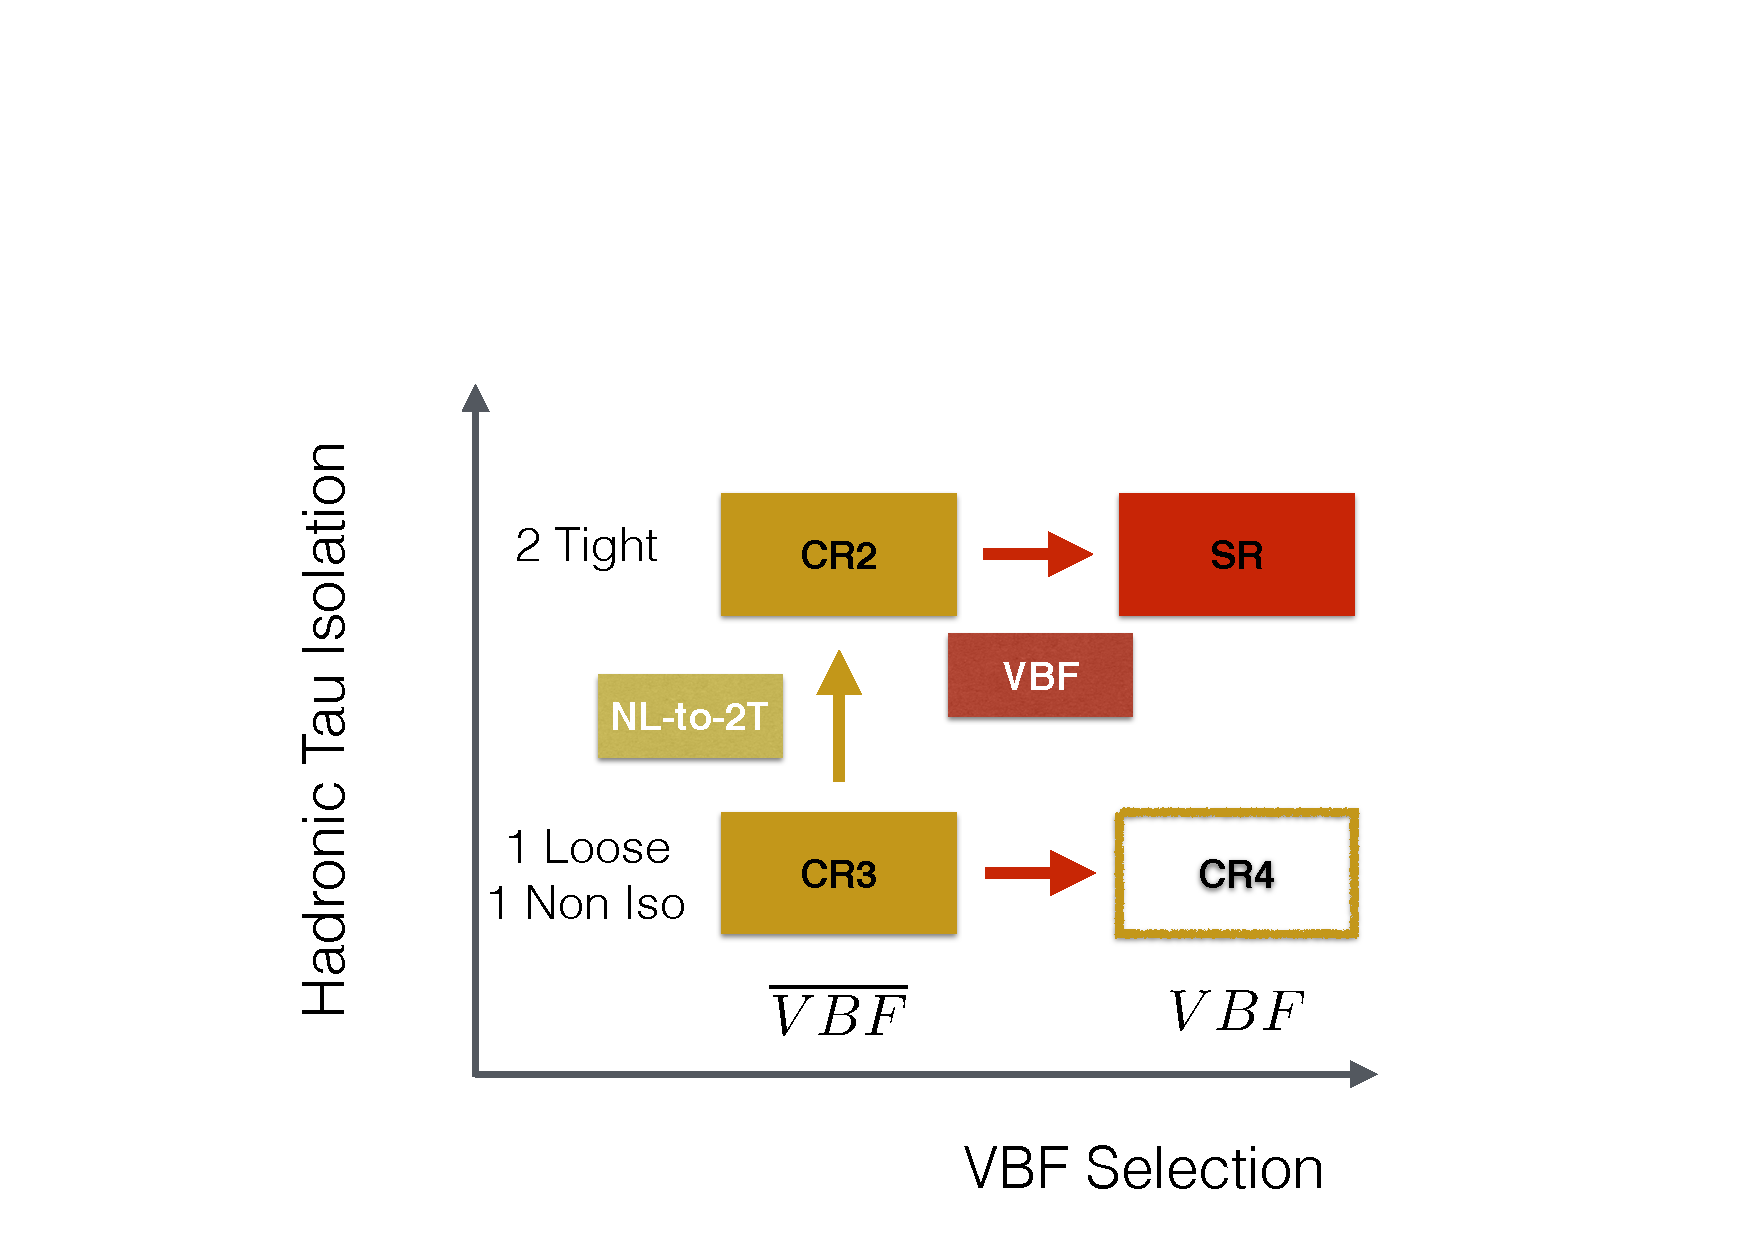
\includegraphics[width=0.75\textwidth]{PLOTS/diTauHadLSotherPlots/controlregions13TeV.pdf}
	\end{tabular}
	\caption{Definition of Signal and Control Regions using different $\hadtau$ isolation criteria and VBF selection.}
	\label{fig:crs_13tev}
\end{figure}

\begin{figure}[tbh!]
	\centering
	\begin{tabular}{cc}
		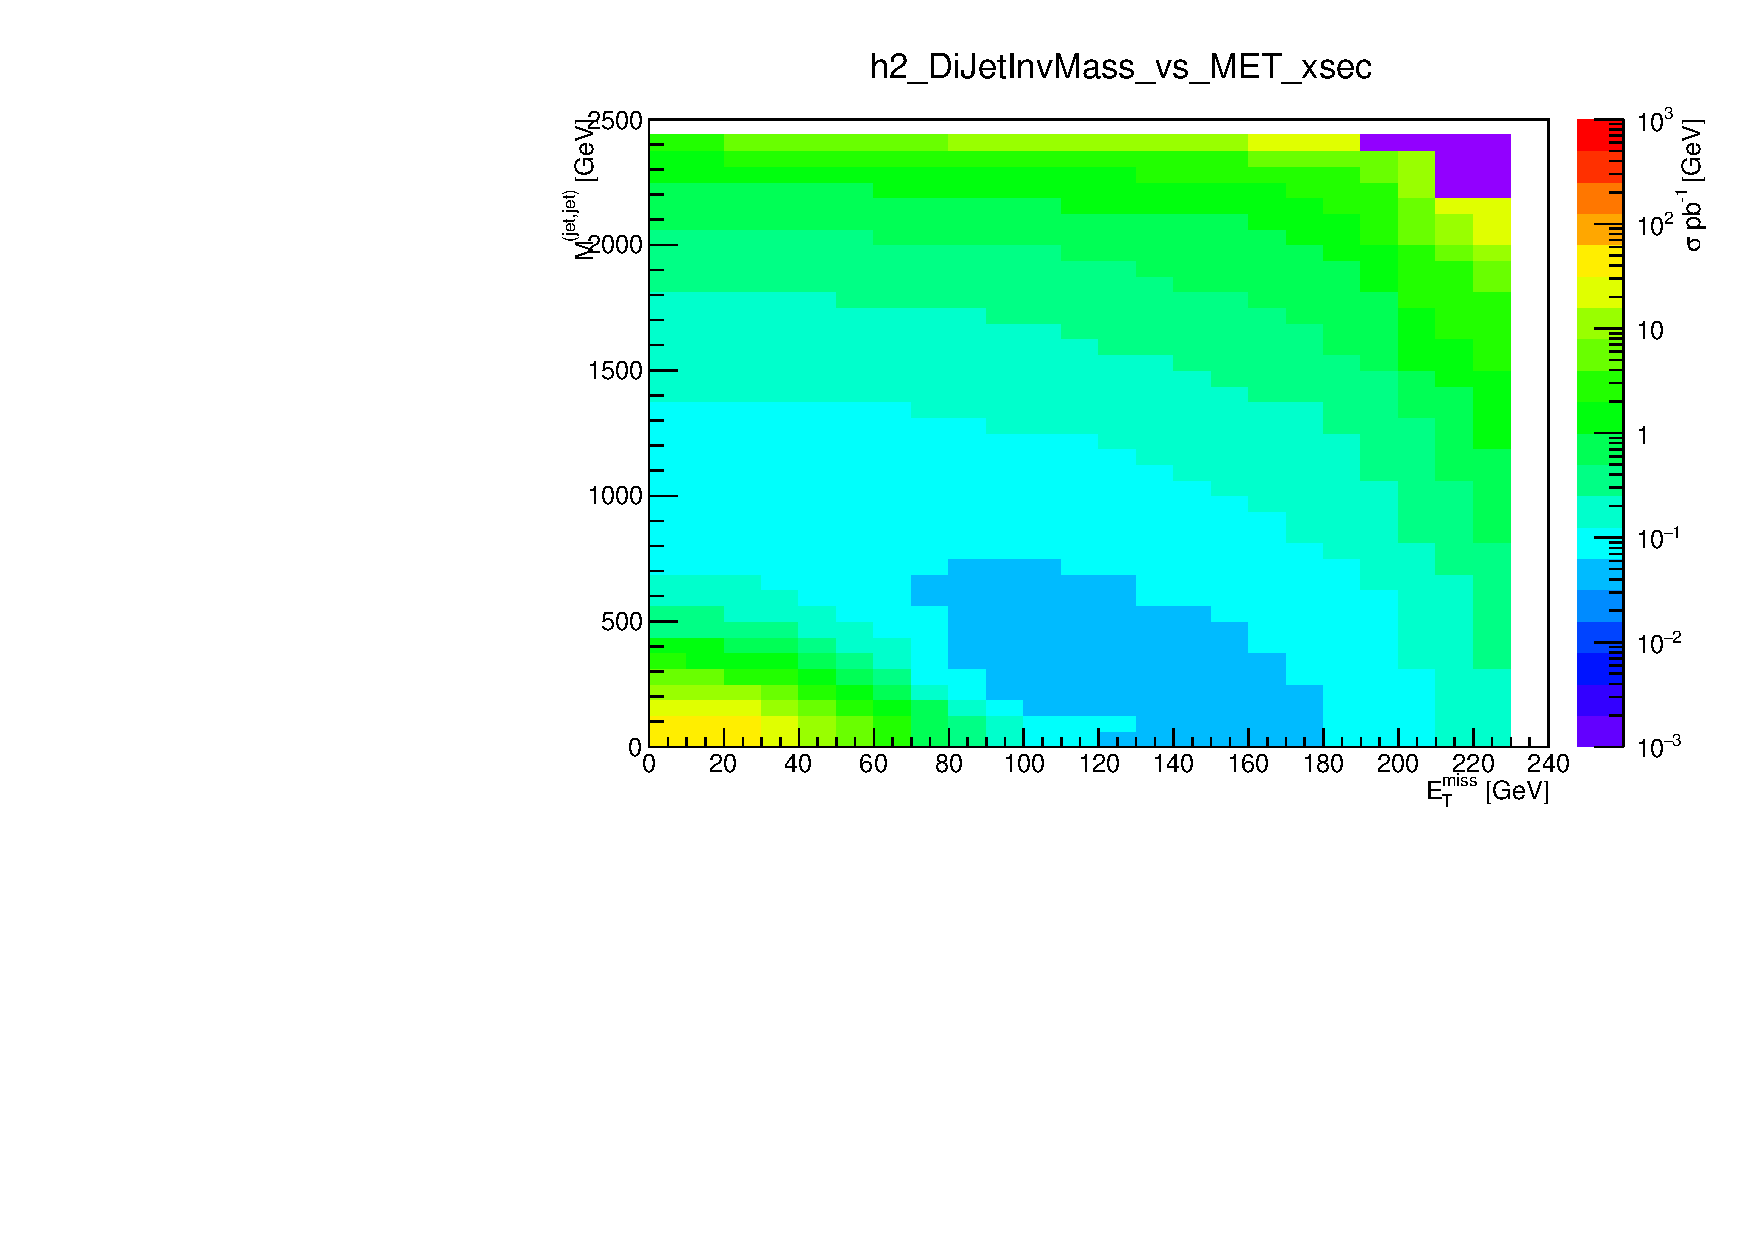
\includegraphics[width=0.48\textwidth]{analysis/pics/chi300_stau295_LSP0_taupt20.pdf}
		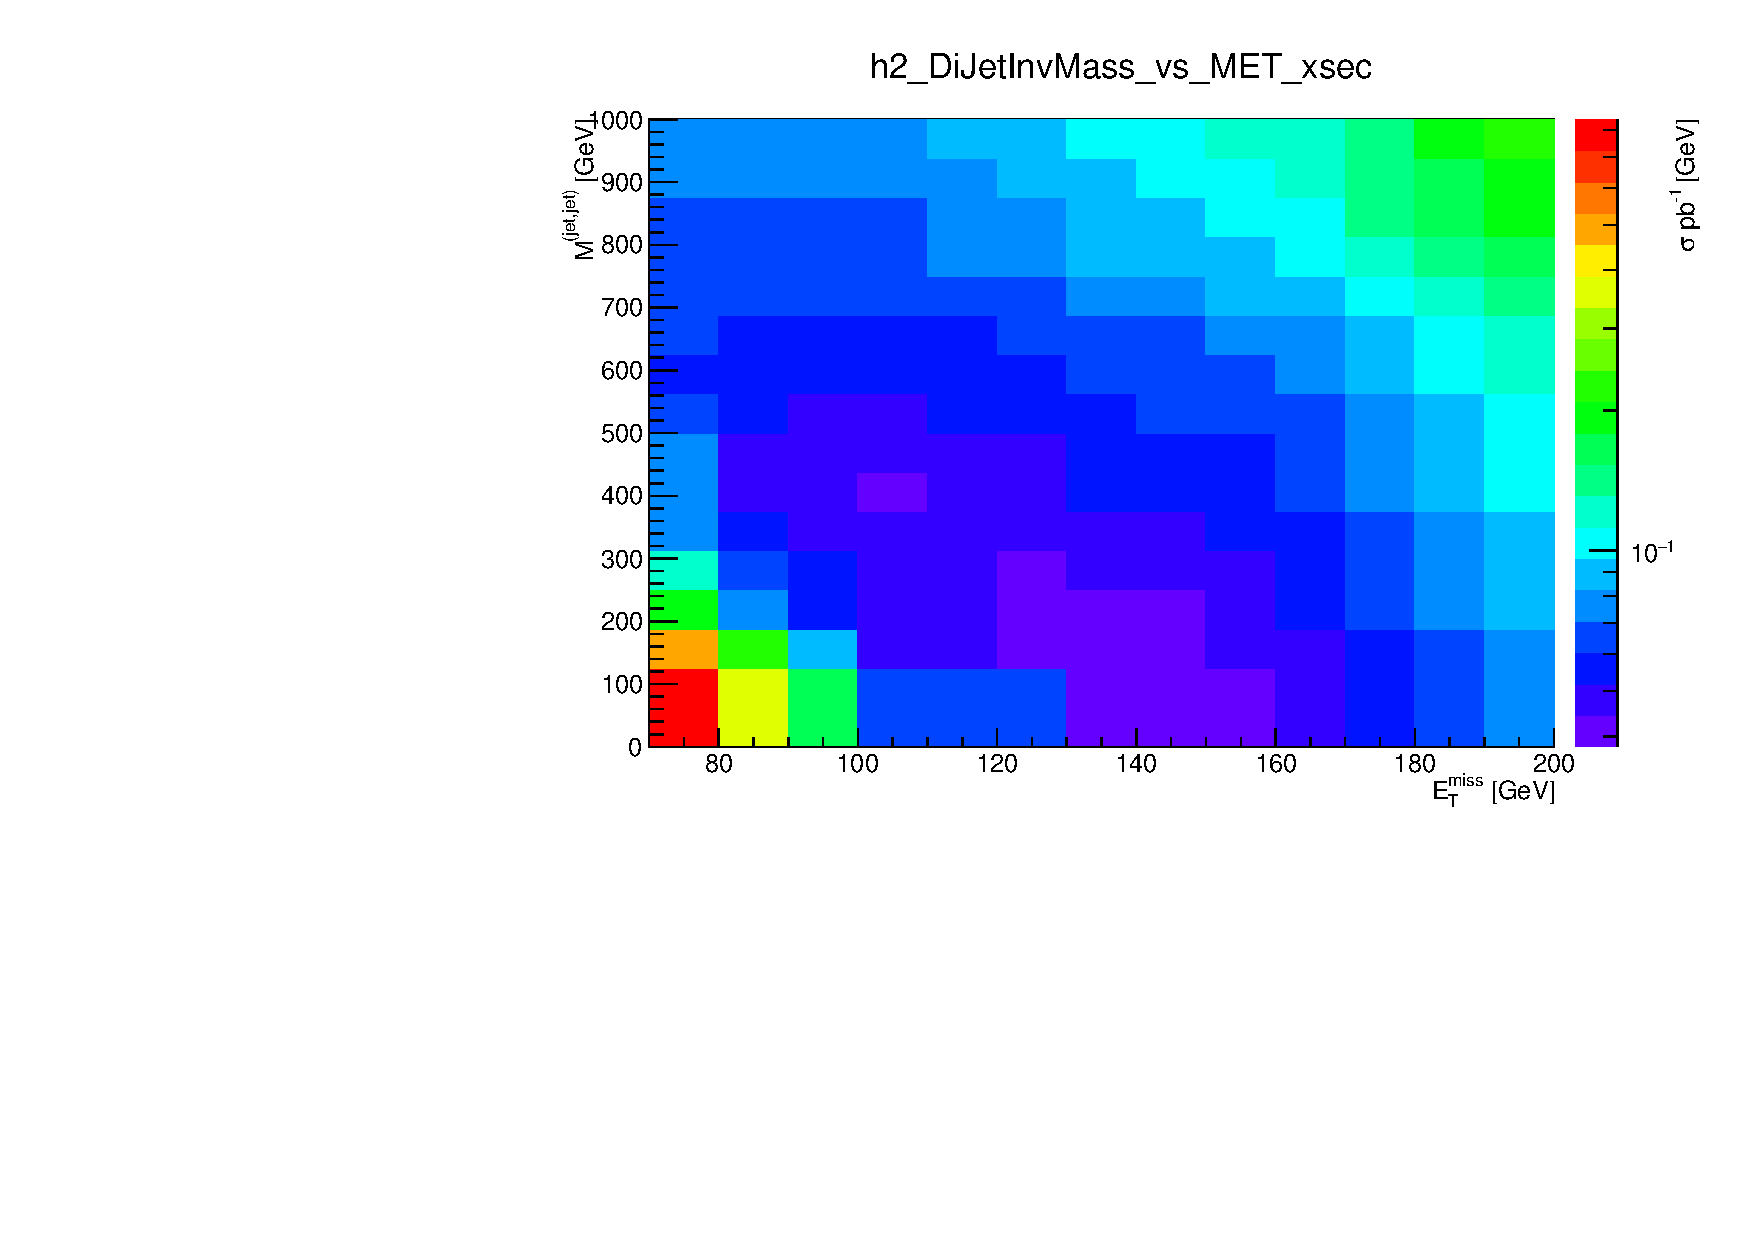
\includegraphics[width=0.48\textwidth]{analysis/pics/chi300_stau295_LSP0_taupt20_zoom.pdf} 		
	\end{tabular}
	\caption{chi300\_stau295\_LSP0\_taupt20}
\end{figure}

\begin{figure}[tbh!]
	\centering
	\begin{tabular}{cc}
		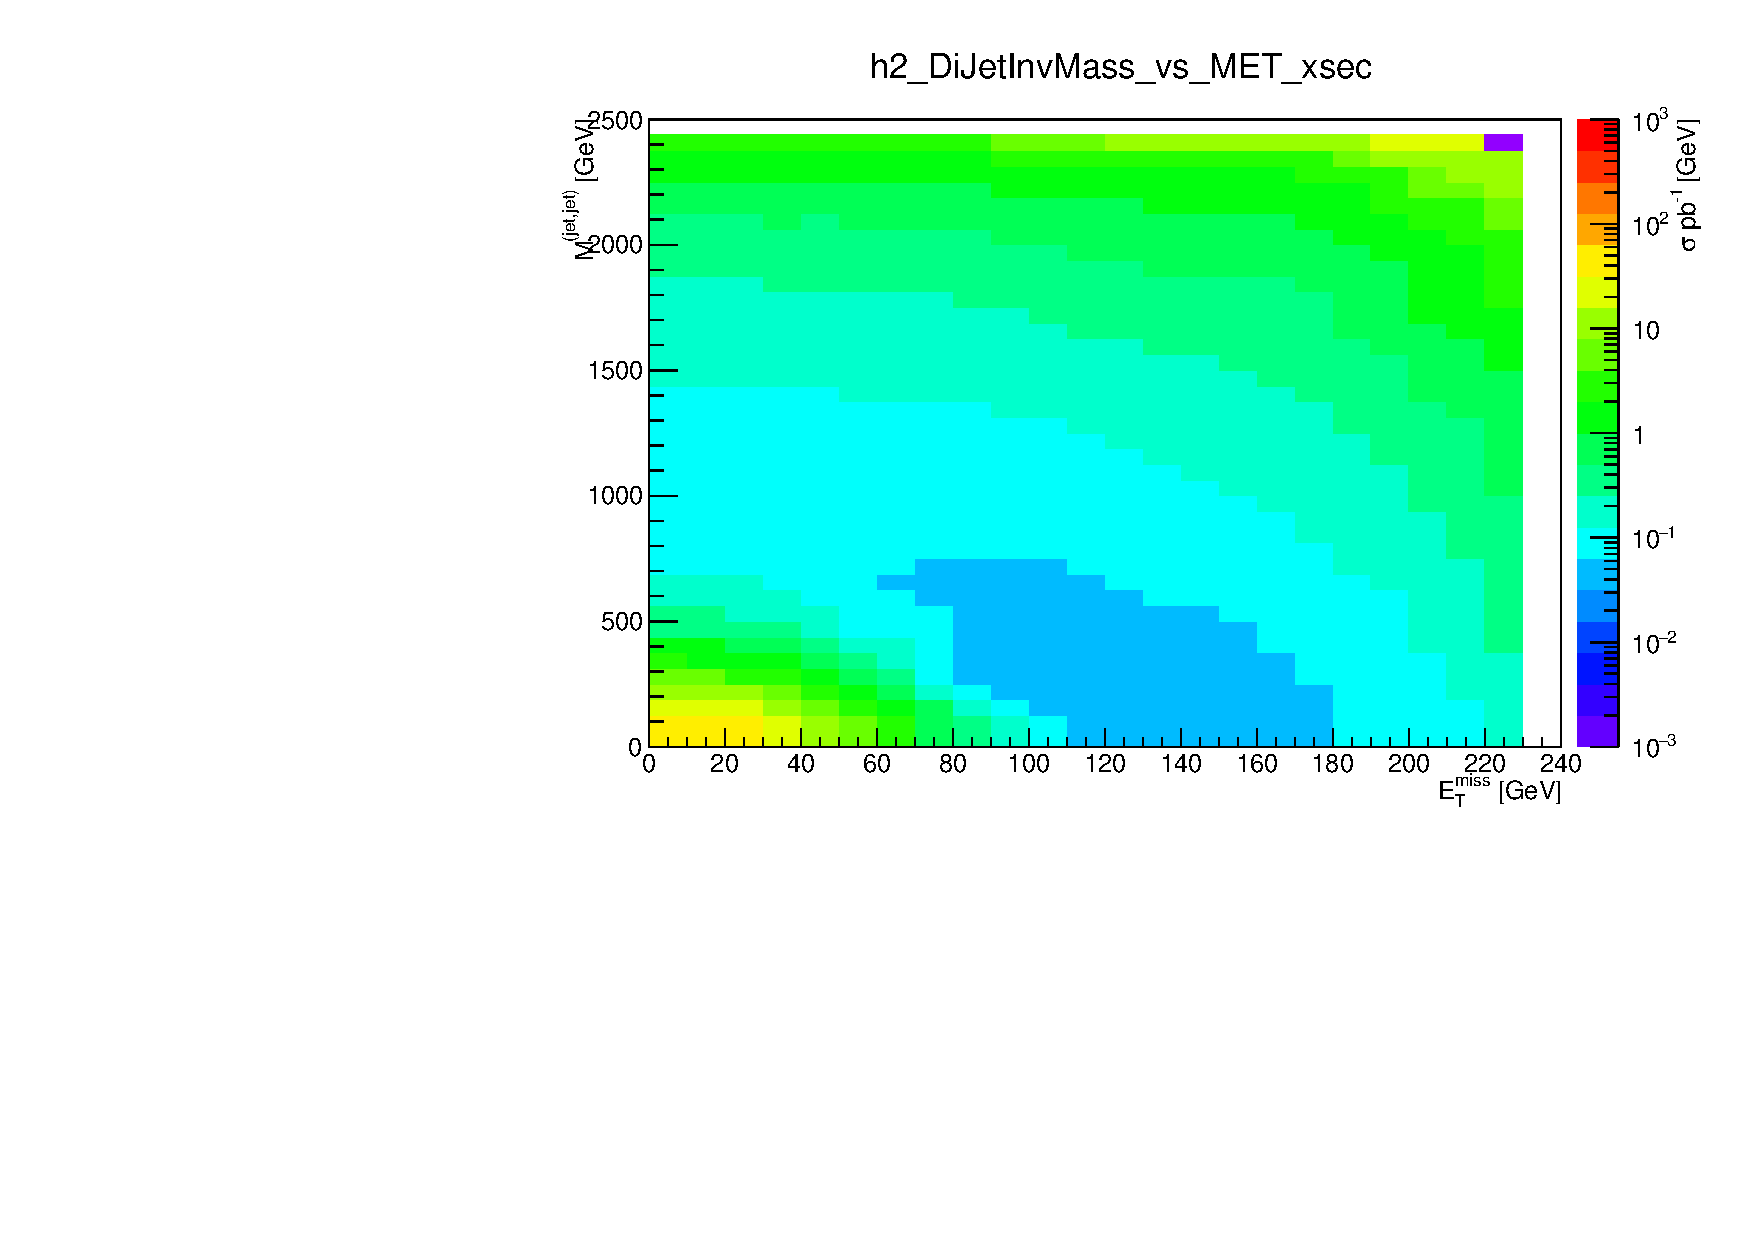
\includegraphics[width=0.48\textwidth]{analysis/pics/chi200_stau195_LSP0_taupt20.pdf}
		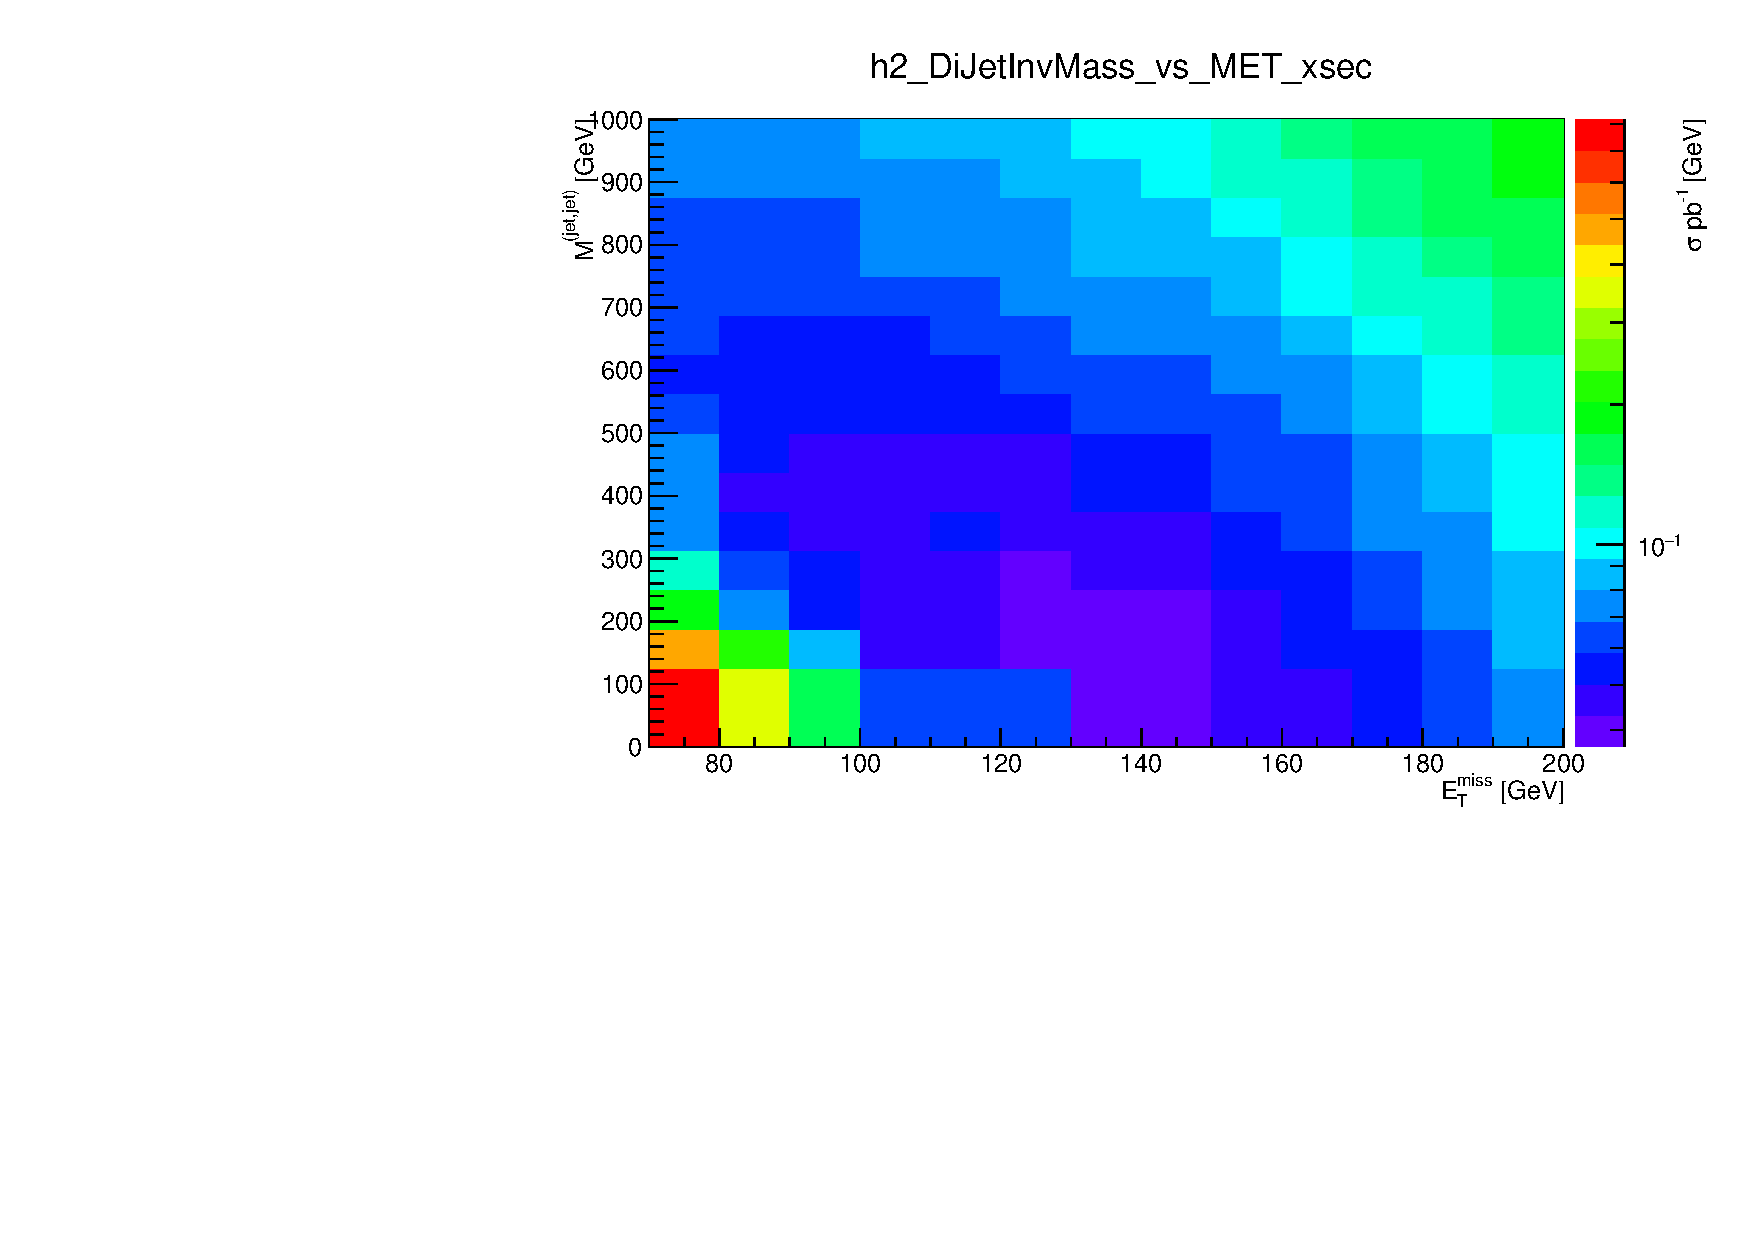
\includegraphics[width=0.48\textwidth]{analysis/pics/chi200_stau195_LSP0_taupt20_zoom.pdf} 		
	\end{tabular}
	\caption{chi200\_stau195\_LSP0\_taupt20}
\end{figure}

\begin{figure}[tbh!]
	\centering
	\begin{tabular}{cc}
		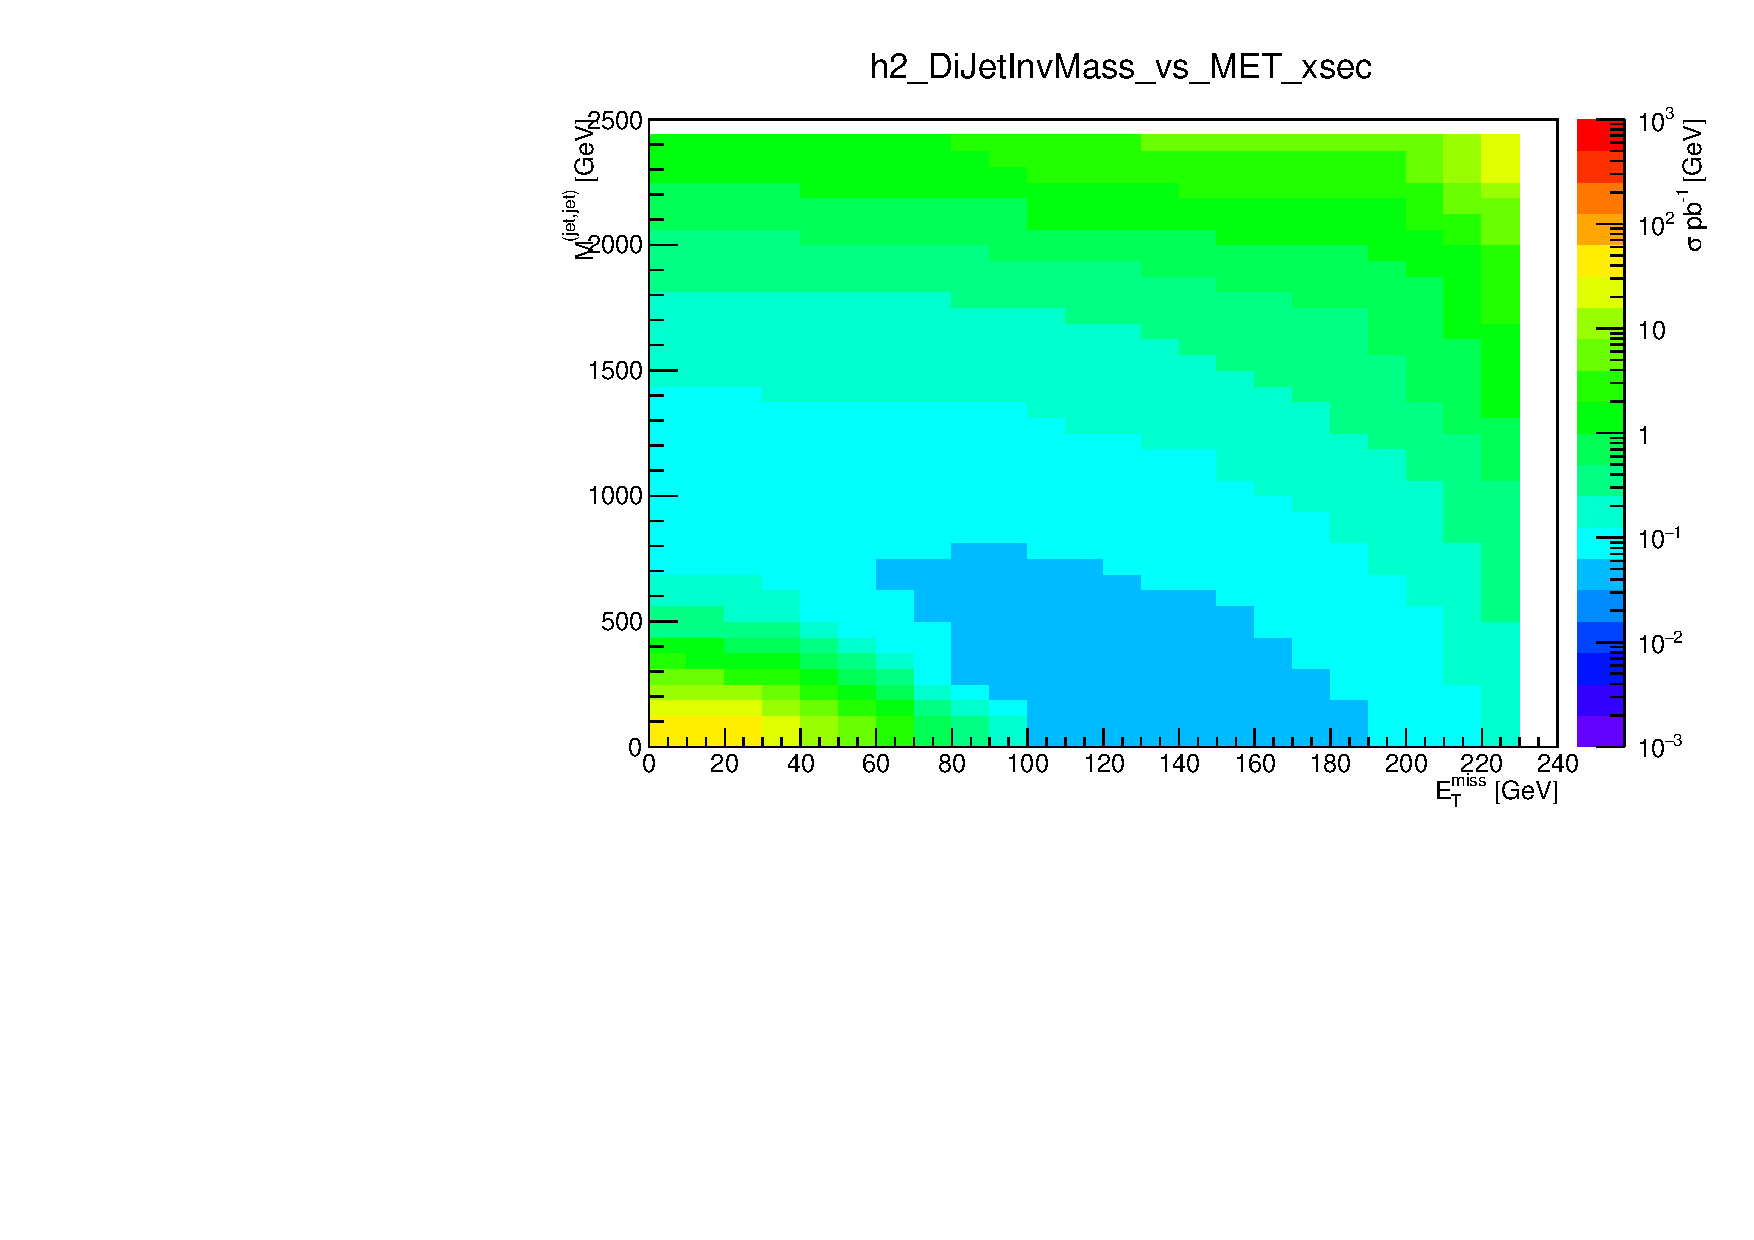
\includegraphics[width=0.48\textwidth]{analysis/pics/chi100_stau095_LSP0_taupt20.pdf}
		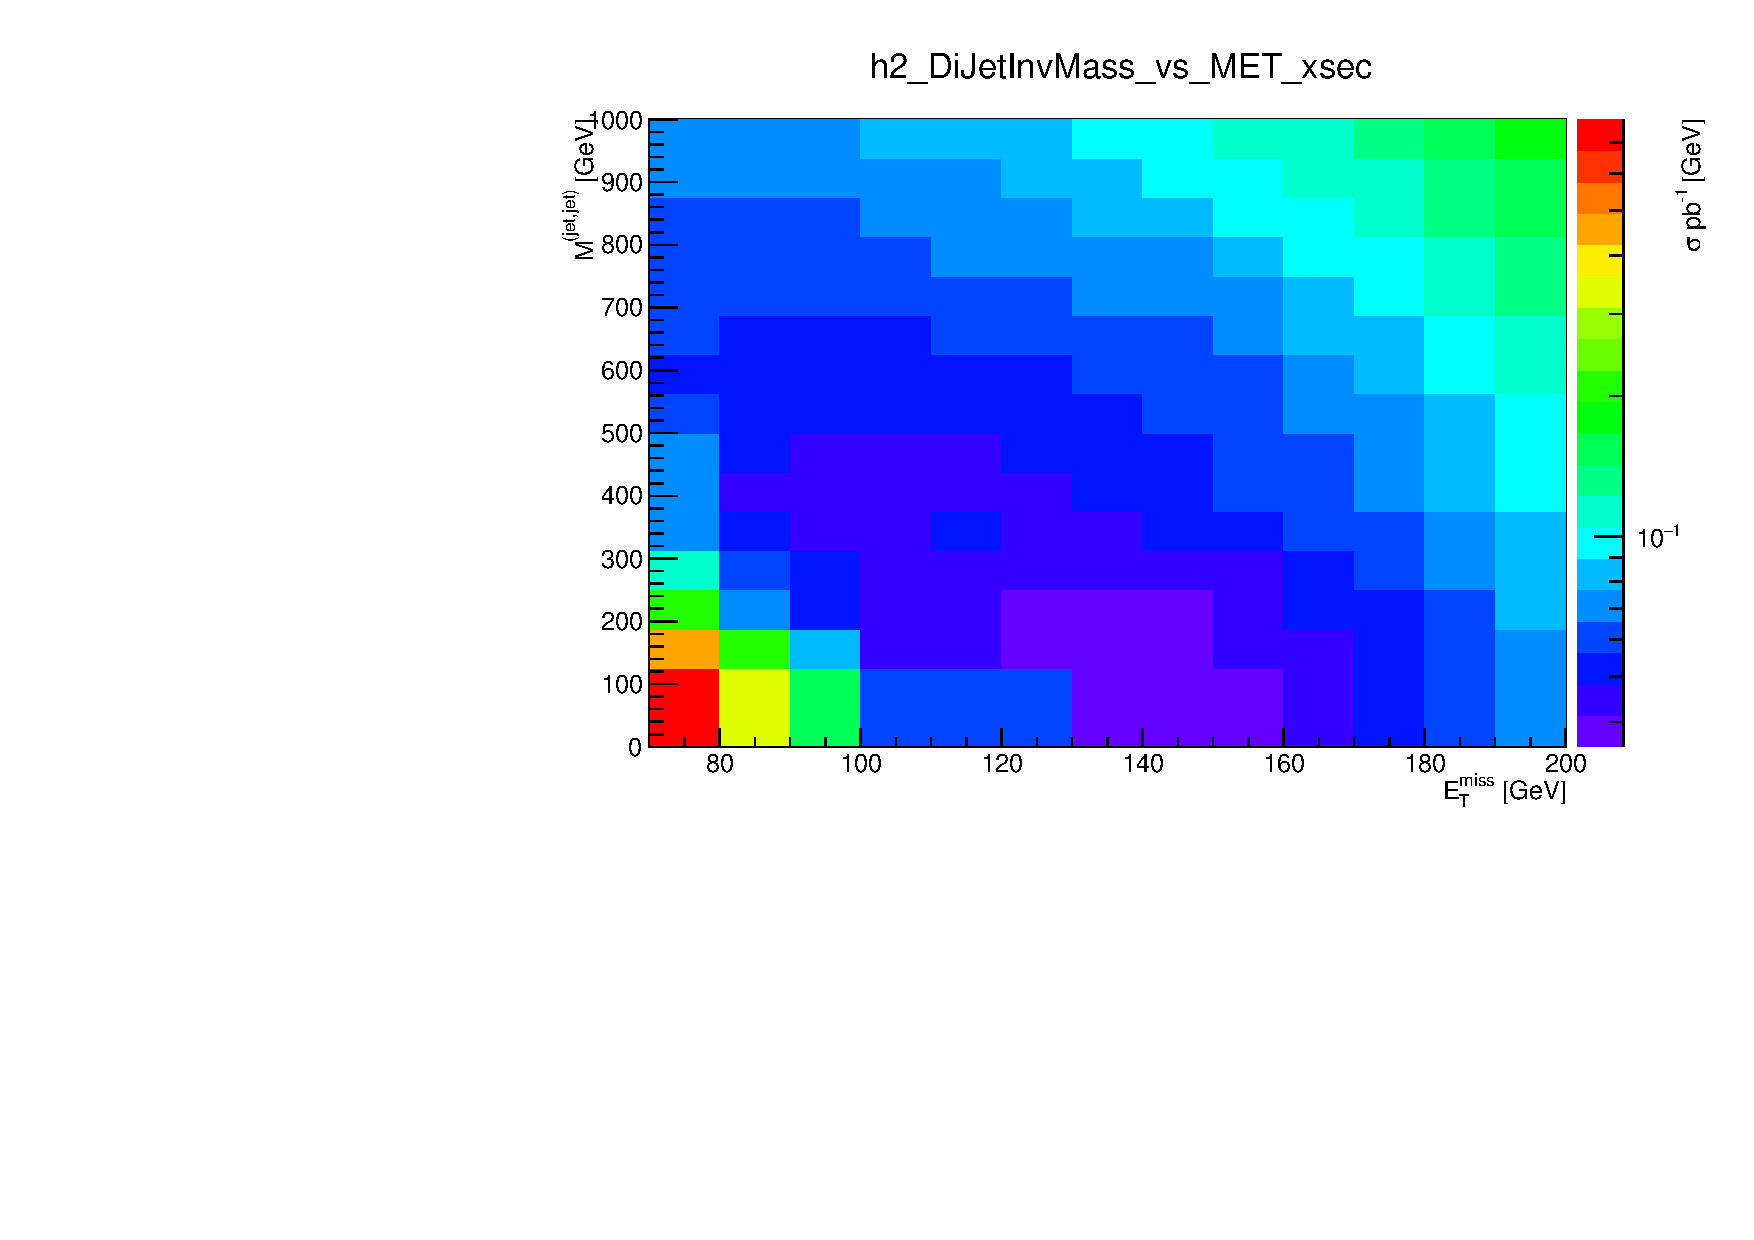
\includegraphics[width=0.48\textwidth]{analysis/pics/chi100_stau095_LSP0_taupt20_zoom.pdf} 		
	\end{tabular}
	\caption{chi100\_stau095\_LSP0\_taupt20}
\end{figure}
